%-------------------------------------------------------------------------------------------------------
%-------------------------------------------------------------------------------------------------------
\chapter{RtLib Storage}

All data of a LCS node is kept in volatile \texttt{(MEM)} and non-volatile \texttt{(NVM)}. The data is structured into several data areas which we call **map**s. A map is a memory area which can be found in MEM and NVM or only in MEM. The key idea is that a map in MEM is initialized from its NVM counterpart at runtime start. Changes in a MEM map can be synced with its NVM map counterpart. There are also maps that do not have a NVM counterpart. These maps are initialized with default values defined for this map. 

Maps do of course have a size. A port map for example will have a number of entries, one for each port. The design choice was whether all map sizes are configurable or rather a fixed size. The current design features a fixed size scheme. There are a few key reasons for this decision. First, there is no configuration need when initializing a node. Second, the total size even when generously sizing the maps is rather small compared to what the hardware can do. A node with 64 node attribute, 15 ports each of which also have 64 port attributes, an event map of 1024 events to manage and space for some miscellaneous date items will be around 8 Kbytes of data. A node with a 32K NVM chip still has plenty of space for user data. A raspberry Pi PICO has 264Kbytes of MEM, so also not an issue. Finally, with a fixed map layout, the NVM data can be copied in one swoop to a memory area on runtime start or reset. 

This chapter presents a high level overview of the available maps and their purpose. Instead of painting many pictures, we will directly take code snippets from the runtime include files to show the data found in each map. Note that all maps are only accessible via runtime library routines.

\section{Node Map}

The node map is a node private data structure only accessible to the library firmware. It contains the information about the configured maps, the node options, nodeId, canId and other data such as the library version. When a node is initially created the configuration descriptor contains all the required information to set up a node map. Nodes need volatile and non-volatile storage. Our design implements a mirroring scheme. For the LCS storage there is a memory and an EEPROM version with the same layout. When a node is running the memory version is the storage to use for performance reasons. Also, it can be expected that the memory contents changes very often during operation. EEPROMs do have a limited number of writes in their lifetime and are not that performant for a write cycle. On the other the other hand the data is stored non-volatile. Information that needs to be changed and available across a restart is therefore synced from MEM to NVM. On restart, the NVM data is just copied to MEM. We always start with a defined state. The following figure shows the nodeMap data structure.


picture: the high level structure of the node map...

\begin{figure}[!ht]
    \centering
   % 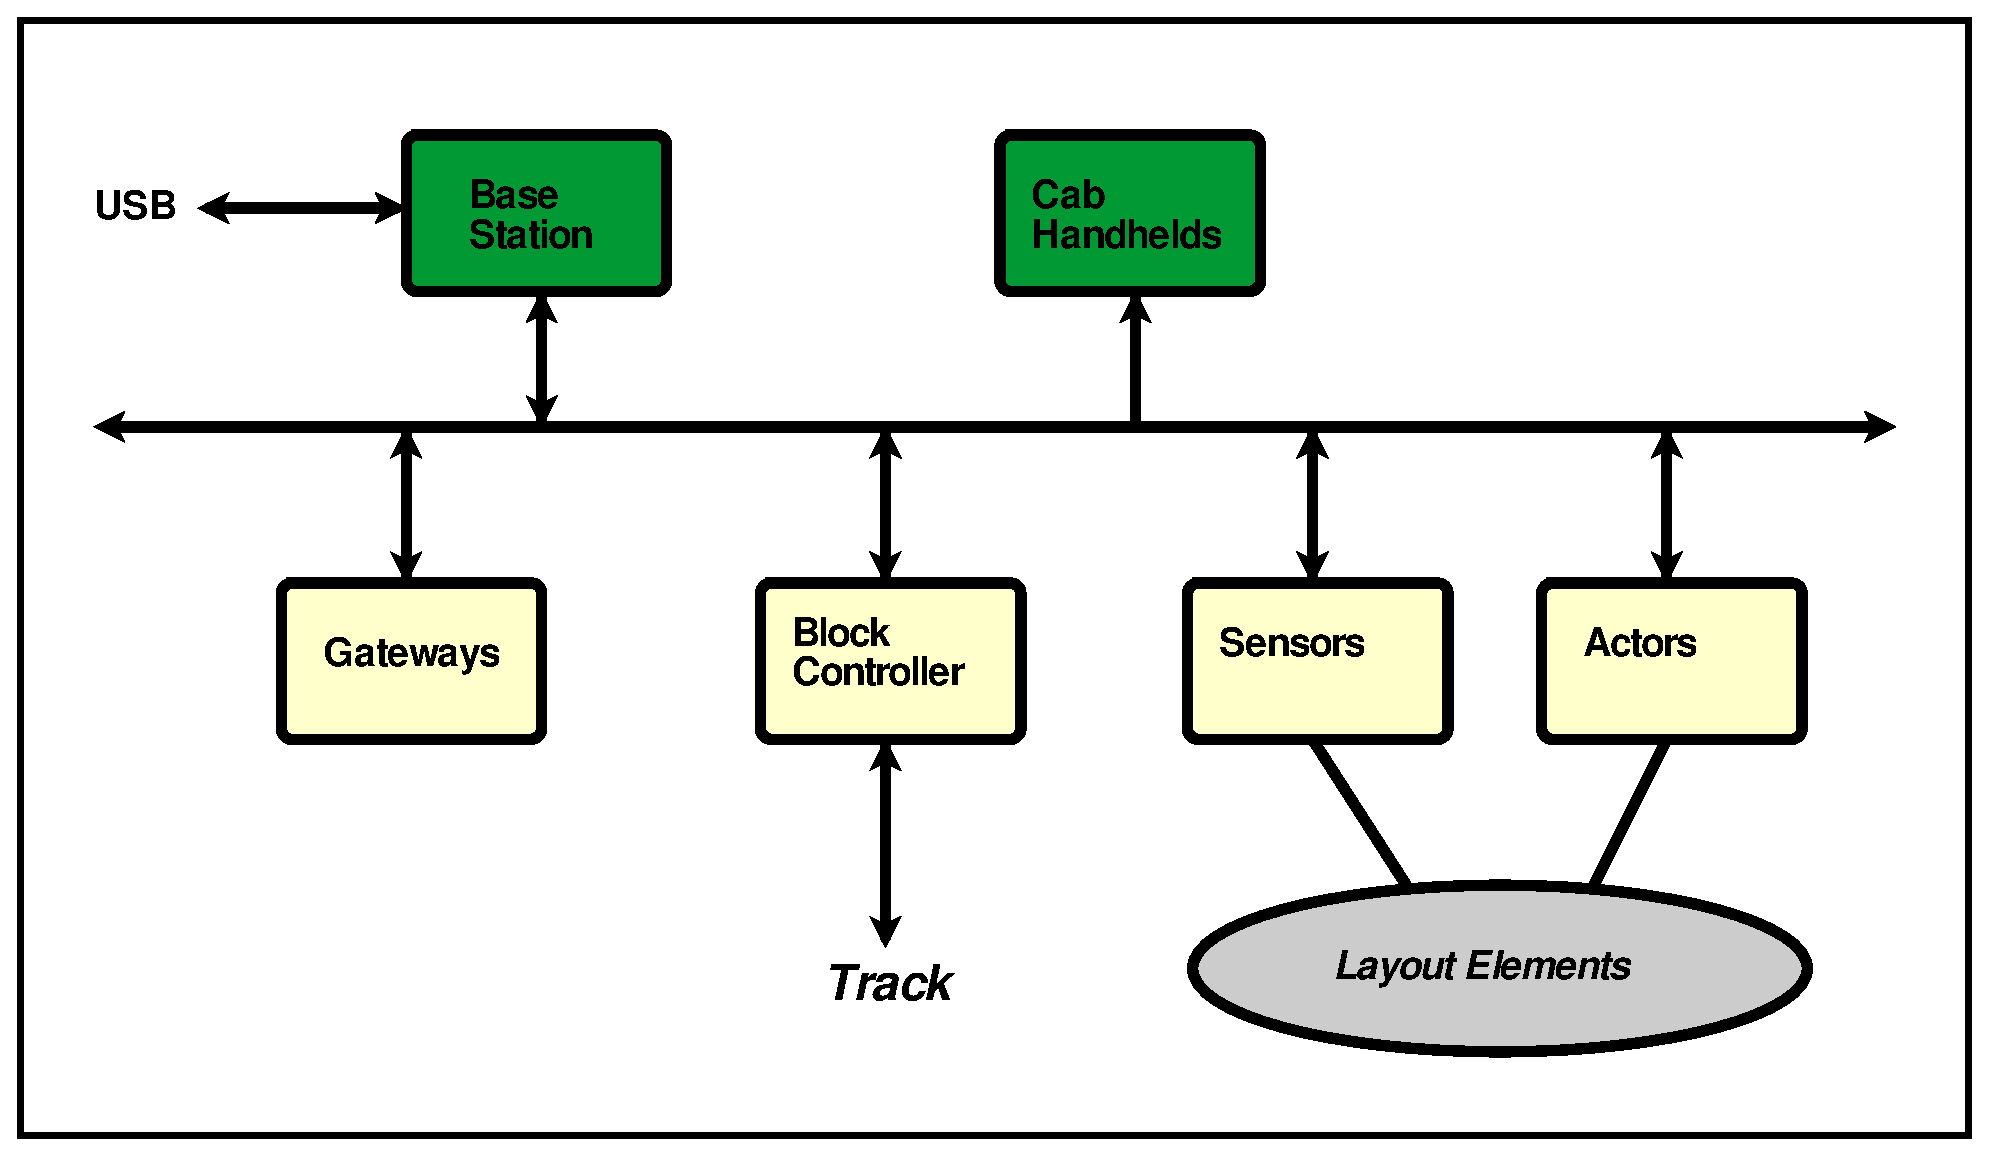
\includegraphics[page=1, width=\textwidth]{./figures/Schematic_LcsNodes-Layout-Overview.pdf}
   %![Schematic_LcsNodes-Core-Library-Overview.png](./Figures/Schematic_LcsNodes-Core-Library-Overview.png )
\end{figure}

Most of the data items deal with the location and entry sizes of the key maps. In addition, there are the nodeId, the node name, creation options, actual status flags and the set of node map attributes. Finally, the software version of the node version is kept here. For the firmware programmer there are methods to read from and write an item to the node. The library the \textbf{nodeGet}, \textbf{nodePut} and \textbf{nodeReq} routines offer a controlled access to the node map and other node data for node firmware programmers. They both use an item / value concept. Each routine passed an item Id for the data of interest and the data value. We will see an example later in this chapter. There are also three LCS messages, \texttt{(QRY-NODE)}, \texttt{(REP-NODE)} and \texttt{(SET-NODE)} which allow for access from another node. Since these messages come from another node, there is also the option to register a callback for access control checks to node data before the operation is performed.

\section{Port Map}

The port map is an array of port map entries. The maximum number of ports are set through the node configuration descriptor values set by the firmware programmer. Changing the number of ports results in a node re-initialization, rebuilding the port map and all non-volatile port map data lost. During runtime there is a non-volatile and a memory version of this map. On node startup or reset, the non volatile port map entries are copied to their memory counterpart.

\lstset{language=c++, style=codesnippetstyle}
\begin{lstlisting}
struct LcsPortMapEntry {

  
};
\end{lstlisting}

The port map entry contains flags that describe the port configuration options and the current operational setting. The event handling fields hold for an inbound port the current event received, the action and value as well as the a possible time delay before invoking the callback. For an outbound port the event fields describe the event to send when the condition for sending that event is encountered. The port map entries are located by just indexing into the port map.

The library \textbf{nodeGet}, \textbf{nodePut} and \textbf{nodeReq} routines presented before, offer a controlled access to the port map entry. The item and portId passed determine whether a node or port item is requested. Depending on the item, a portId of 0 will refer to all ports on the node or the node itself.

\section{Node and Port Items}

The term "item" came up numerous times by now. Nodes and ports features to access their attributes through an \textbf{item Id}. An item Id is just a number in the range from 1 to 255. Here is the definition from the library include file. The include file also contains the item numbers for the reserved node info and control items.

\begin{table}[h!]
    \begin{center}
        \caption{Item ranges}
        \begin{tabular}{|l|l|p{0.72\textwidth}|}
            \toprule
            \textbf{Low} & \textbf{High} & \textbf{Purpose} \\
            \midrule
            0 & & NIL Item \\
            \midrule
            1 & 63 & Reserved items for node and ports \\
            \midrule
            64 & 127 & user defined items passed to the registered callback function \\
            \midrule
            128 & 191 & Node or Port Attributes first copied from NVM to MEM and then returned \\
            \midrule
            192 & 255 & Node or Port Attributes first copied from NVM to MEM and then returned \\
            \bottomrule
        \end{tabular}
    \end{center}
\end{table}

The first set of item numbers are reserved by the core library itself for node and port items that are standardized across all nodes. The range 64 to 127 and 128 to 191 describes the set of node or port attributes. The two groups actually represent the same attributes. For example the item number 64 refers to the same attributes as item 128 does. The difference is that the latter group also accesses the NVM storage. Items 192 to 255 are completely user defined. Using these numbers will just result in a callback invocation. Note that a callback can do anything. For example, turning a signal on or off could be an item Id of let's say 205 and sending a node control message with the item 205 and the value of 1 in the first argument would result in invoking a callback which implements how to turn the signal on. In short, a node supports variable access, comparable to the CV concept in DCC, and also a function call concept which allows a great flexibility for the firmware programmer.

\section{Event Map}

The event map is an array of event map entries, each containing the eventId that node is interested in and the port Id to inform when the event is encountered. The maximum number of event map entries is set through the node configuration descriptor values set by the firmware programmer. When a new node is configured, this value is used to construct the empty event map. Any change of this value results in a node re-initialization of the node, rebuilding the event map with all non-volatile event map data lost.

\lstset{language=c++, style=codesnippetstyle}
\begin{lstlisting}
struct LcsEventMapEntry {

    uint16_t	eventId;
    uint16_t 	portId;
};
\end{lstlisting}

??? explain the SYNC approach for this map...

Like all other maps, the event map is stored in two places. The non-volatile version of the eventMap is an array of event map entries. Whenever a new entry is added, a free entry is used to store this information. The memory version of the event map is a sorted version of all used non-volatile entries. The entries are first sorted by event Id. For entries with the same event Id, the port Id is then sorted in ascending order.

In addition to the search function, event map entries can be added and deleted by specifying the eventId and portId. EventMap entries can also be accessed by their position in the event map. This is necessary to read out the event map for example though a configuration tool. While reading an event map entry from the event map is supported in both node configuration and operation mode, deleting or adding an entry is only supported in node configuration mode.

\section{User defined maps}

In addition to the runtime maps for node, ports, and events, the LCS runtime offers a user map for the firmware to use. This storage area is simply an unstructured array and the size depends on the capability of the node hardware NVM storage size. The area is the remaining storage available in the NVM chip array.

 ??? explain the concept and purpose ...

 \section{Periodic task Map}

\lstset{language=c++, style=codesnippetstyle}
\begin{lstlisting}

    User map \dots

\end{lstlisting}

 \section{Pending Request Map}

The pending request map, is a small map that keeps track of outstanding reply messages to a previously issued message request. If a node sends a request, an entry is added to this map that indicates that a reply from another node is pending. When a reply messages is detected, the firmware callback is only invoked if this reply matches a previous request. This map is a volatile structure, a restart will clear all outstanding requests.

??? a timeout concept

\section{Driver function map}

\lstset{language=c++, style=codesnippetstyle}
\begin{lstlisting}

... code snippet here ...

\end{lstlisting}

\section{Driver map}

for extension boards to be explained later...

\lstset{language=c++, style=codesnippetstyle}
\begin{lstlisting}

... code snippet here ...

\end{lstlisting}

\section{Summary}

??? explain again why this NVM is key and thus important...

To summarize, node storage is organized in maps. 

There is the node map, which is the global place for locating all other areas in the node. The port map contains the data for the configured ports. The event map is the mapping mechanism for events to ports. During node startup, the non-volatile data is copied to a newly allocated memory area. After initialization the node will only work from the memory area. All read and write operations use the memory storage area. When setting a value in any map, the flush option allows for setting its non-volatile counter part as well, so that we have a new initial value for the next restart.

Any change to the structure of the maps, for example changing the number of entries in a map, but also a different size of a data structure caused by a new library version, will result in a rebuilding of the non-volatile memory area with all previous data lost. The layout configuration data, such as the mapping of events to the node and port needs to be stored for example in a computer system so that can be reloaded once a node is re-created. A node has no way of keeping stored data across structural changes to its map layout.
